\documentclass[14pt]{beamer}
\usepackage{pgf,pgfpages,amsmath,booktabs,fancyvrb,animate,graphicx,bera,bm,ragged2e}
\usepackage[australian]{babel}
\usepackage[utf8]{inputenc}
%\usepackage{abs}
\usepackage{tikz}
\usetikzlibrary{trees,shapes,arrows,matrix}

\usetheme{Monash}

\usepackage{eurosym,dcolumn,xmpmulti,booktabs}
\usepackage{bbding,color}

\def\biz{\begin{itemize}[<+-| alert@+>]}
\def\eiz{\end{itemize}}
\def\ben{\begin{enumerate}[<+-| alert@+>]}
\def\een{\end{enumerate}}

\def\hl{\color[RGB]{6,84,182}}

\def\E{\text{E}}
\def\V{\text{Var}}
\def\up#1{\raisebox{-0.3cm}{#1}}
\def\AICc{\text{AIC$_{\text{c}}$}}
\def\pred#1#2#3{\hat{#1}_{#2|#3}}
%\setbeamerfont{title}{size=\Large,series=\bfseries}

\def\h+{h_{m}^{+}}
\def\NID{\stackrel{\mbox{\scriptsize iid}}{\sim}\mbox{N}}
\def\var{\text{Var}}
\def\E{\text{E}}
\def\damped{$_{\text{\footnotesize d}}$}
\def\logN{\text{logN}}
\def\N{\text{N}}
\newcolumntype{.}{D{.}{.}{-1}}
\def\bbeta{\bm{\beta}}
\def\bY{\bm{Y}}
\def\bS{\bm{S}}
\def\bJ{\bm{J}}
\def\bSigma{\bm{\Sigma}}
\def\bOmega{\bm{\Omega}}
\def\bLambda{\bm{\Lambda}}
\def\bJ{\bm{J}}
\def\mc{\multicolumn}
\def\0{\phantom{0}}
\def\bI{\text{\rm\textbf{I}}}
\def\by{\bm{y}}

\input header.tex

% BIBLIOGRAPHIES
\usepackage[style=authoryear,bibencoding=utf8,minnames=1,maxnames=4, maxbibnames=99,natbib=true,dashed=false,terseinits=true,giveninits=true,uniquename=false,uniquelist=false,labeldate=true,doi=false, isbn=false, natbib=true,backend=biber]{biblatex}

\DeclareFieldFormat{url}{\url{#1}}
\DeclareFieldFormat[article]{pages}{#1}
\DeclareFieldFormat[inproceedings]{pages}{\lowercase{pp.}#1}
\DeclareFieldFormat[incollection]{pages}{\lowercase{pp.}#1}
\DeclareFieldFormat[article]{volume}{\mkbibbold{#1}}
\DeclareFieldFormat[article]{number}{\mkbibparens{#1}}
\DeclareFieldFormat[article]{title}{\MakeCapital{#1}}
\DeclareFieldFormat[article]{url}{}
\DeclareFieldFormat[Techreport]{Url}{}
\DeclareFieldFormat[book]{url}{}
\DeclareFieldFormat[inbook]{url}{}
\DeclareFieldFormat[incollection]{url}{}
\DeclareFieldFormat[inproceedings]{url}{}
\DeclareFieldFormat[inproceedings]{title}{#1}
\DeclareFieldFormat{shorthandwidth}{#1}
%\DeclareFieldFormat{extrayear}{}
% No dot before number of articles
\usepackage{xpatch}
\xpatchbibmacro{volume+number+eid}{\setunit*{\adddot}}{}{}{}
% Remove In: for an article.
\renewbibmacro{in:}{%
  \ifentrytype{article}{}{%
  \printtext{\bibstring{in}\intitlepunct}}}

\AtEveryBibitem{\clearfield{month}}
\AtEveryCitekey{\clearfield{month}}

\bibliography{rjhpubs,Rpackages}


\title{Probabilistic Hierarchical Forecasting}
\author{Rob J Hyndman}
\date{}


\begin{document}

\begin{frame}
\titlepage
\end{frame}




\section{Temporal hierarchies}

\begin{frame}{Temporal hierarchies}\vspace*{-0.2cm}

\begin{center}
%\begin{minipage}{9.6cm}
%\begin{block}{}
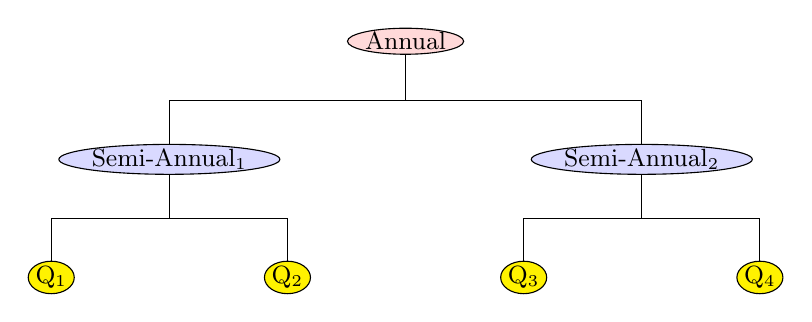
\begin{tikzpicture}
\tikzstyle{every node}=[ellipse,draw,inner sep=0.2pt,fill=red!15,font=\small]
\tikzstyle[level distance=.1cm]
\tikzstyle[sibling distance=7cm]
\tikzstyle{level 1}=[sibling distance=60mm,font=\small,set style={{every node}+=[fill=blue!15]}]
\tikzstyle{level 2}=[sibling distance=30mm,font=\small,set style={{every node}+=[fill=yellow]}]
\tikzstyle{level 3}=[sibling distance=10mm,font=\small,set style={{every node}+=[fill=green]}]
\node{Annual}[edge from parent fork down]
 child {node {Semi-Annual$_1$}
   child {node {Q$_1$}
%     child {node {M$_1$}}
%     child {node {M$_2$}}
%     child {node {M$_3$}}
   }
   child {node {Q$_2$}
%     child {node {M$_4$}}
%     child {node {M$_5$}}
%     child {node {M$_6$}}
   }
 }
 child {node {Semi-Annual$_2$}
   child {node {Q$_3$}
%     child {node {M$_7$}}
%     child {node {M$_8$}}
%     child {node {M$_9$}}
   }
   child {node {Q$_4$}
%     child {node {M$_{10}$}}
%     child {node {M$_{11}$}}
%     child {node {M$_{12}$}}
   }
 };
\end{tikzpicture}
%\end{block}
%\end{minipage}
\end{center}
\pause
\begin{alertblock}{Basic idea:}
\begin{itemize}
\item[\color{white}\ding{229}] Forecast series at each available frequency.
\item[\color{white}\ding{229}] Optimally reconcile forecasts within the same year.
\end{itemize}
\end{alertblock}
\end{frame}


\begin{frame}{Monthly series}\vspace*{-0.5cm}

\only<1>{

\begin{center}
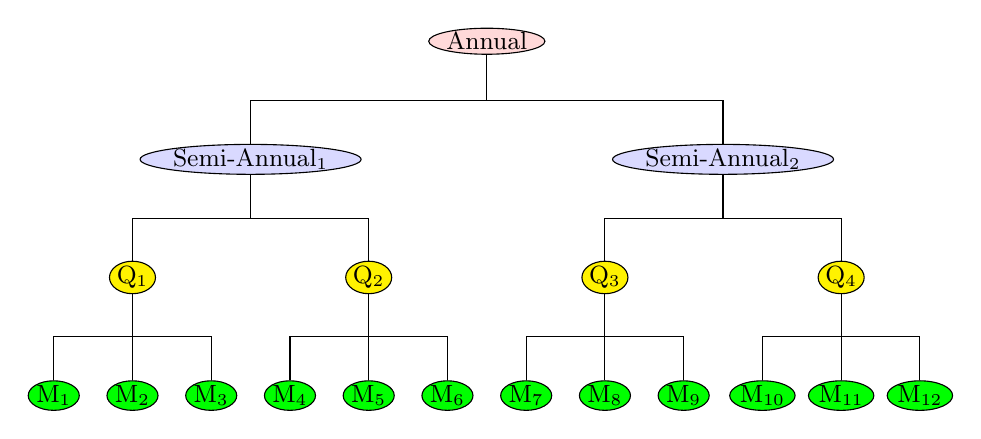
\begin{tikzpicture}
\tikzstyle{every node}=[ellipse,draw,inner sep=0.2pt,fill=red!15,font=\small]
\tikzstyle[level distance=.1cm]
\tikzstyle[sibling distance=7cm]
\tikzstyle{level 1}=[sibling distance=60mm,font=\small,set style={{every node}+=[fill=blue!15]}]
\tikzstyle{level 2}=[sibling distance=30mm,font=\small,set style={{every node}+=[fill=yellow]}]
\tikzstyle{level 3}=[sibling distance=10mm,font=\small,set style={{every node}+=[fill=green]}]
\node{Annual}[edge from parent fork down]
 child {node {Semi-Annual$_1$}
   child {node {Q$_1$}
     child {node {M$_1$}}
     child {node {M$_2$}}
     child {node {M$_3$}}
   }
   child {node {Q$_2$}
     child {node {M$_4$}}
     child {node {M$_5$}}
     child {node {M$_6$}}
   }
 }
 child {node {Semi-Annual$_2$}
   child {node {Q$_3$}
     child {node {M$_7$}}
     child {node {M$_8$}}
     child {node {M$_9$}}
   }
   child {node {Q$_4$}
     child {node {M$_{10}$}}
     child {node {M$_{11}$}}
     child {node {M$_{12}$}}
   }
 };
\end{tikzpicture}
\end{center}}


\only<2->{\begin{center}
%\begin{minipage}{9.6cm}
%\begin{block}{}
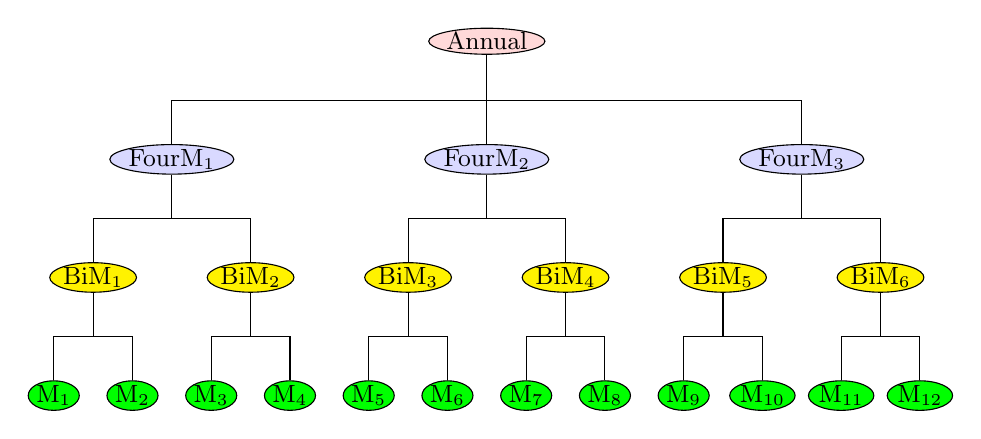
\begin{tikzpicture}
\tikzstyle{every node}=[ellipse,draw,inner sep=0.2pt,fill=red!15,font=\small]
\tikzstyle[level distance=.1cm]
\tikzstyle[sibling distance=7cm]
\tikzstyle{level 1}=[sibling distance=40mm,font=\small,set style={{every node}+=[fill=blue!15]}]
\tikzstyle{level 2}=[sibling distance=20mm,font=\small,set style={{every node}+=[fill=yellow]}]
\tikzstyle{level 3}=[sibling distance=10mm,font=\small,set style={{every node}+=[fill=green]}]
\node{Annual}[edge from parent fork down]
 child {node {FourM$_1$}
   child {node {BiM$_1$}
     child {node {M$_1$}}
     child {node {M$_2$}}
   }
   child {node {BiM$_2$}
     child {node {M$_3$}}
     child {node {M$_4$}}
   }
 }
 child {node {FourM$_2$}
   child {node {BiM$_3$}
     child {node {M$_5$}}
     child {node {M$_6$}}
   }
   child {node {BiM$_4$}
     child {node {M$_7$}}
     child {node {M$_8$}}
   }
 }
  child {node {FourM$_3$}
   child {node {BiM$_5$}
     child {node {M$_9$}}
     child {node {M$_{10}$}}
   }
   child {node {BiM$_6$}
     child {node {M$_{11}$}}
     child {node {M$_{12}$}}
   }
 };
\end{tikzpicture}
%\end{block}
%\end{minipage}
\end{center}}



\biz
\item $k=2,4,12$ nodes
\item $k=3,6,12$ nodes
\item Why not $k=2,3,4,6,12$ nodes?
\eiz
\end{frame}


\begin{frame}{Monthly data}
\fontsize{15}{15}\sf
\hbox{${\underbrace{\footnotesize
\begin{pmatrix}
    A\\
    SemiA_{1}\\
    SemiA_{2}\\
    FourM_{1}\\
    FourM_{2}\\
    FourM_{3}\\
    Q_{1}\\
    \vdots\\
    Q_{4}\\
    BiM_{1}\\
    \vdots\\
    BiM_{6}\\
    M_{1}\\
    \vdots\\
    M_{12}
    \end{pmatrix}}_{(28\times1)}}=
    {\color{red}\underbrace{
    \footnotesize
    \begin{pmatrix}
                1 & 1 & 1 & 1 & 1~~~1~~~1~~~1 & 1 & 1& 1& 1\\
                1 & 1 & 1 & 1 & 1~~~1~~~0~~~0 & 0 & 0& 0& 0\\
                0 & 0 & 0 & 0 & 0~~~0~~~1~~~1 & 1 & 1& 1& 1\\
                1 & 1 & 1 & 1 & 0~~~0~~~0~~~0 & 0 & 0& 0& 0\\
                0 & 0 & 0 & 0 & 1~~~1~~~1~~~1 & 0 & 0& 0& 0\\
                0 & 0 & 0 & 0 & 0~~~0~~~0~~~0 & 1 & 1& 1& 1\\
                1 & 1 & 1 & 0 & 0~~~0~~~0~~~0 & 0 & 0& 0& 0\\
                  &   &   &   & \vdots        &   &  &  &  \\
                0 & 0 & 0 & 0 & 0~~~0~~~0~~~0 & 0 & 1& 1& 1\\
                1 & 1 & 0 & 0 & 0~~~0~~~0~~~0 & 0 & 0& 0& 0\\
                  &   &   &   & \vdots        &   &  &  &  \\
                0 & 0 & 0 & 0 & 0~~~0~~~0~~~0 & 0 & 0& 1& 1\\
                  &   &   &  &  &  &  &  & \\
                \phantom{\vdots}  &   &   &  & \bm{I}_{12} &  &  &  & \\
                  &   &   &  &  &  &  &  & \\
                \end{pmatrix}}_{\bS}}{\color{blue}\underbrace{\small
             \begin{pmatrix}
    M_{1}\\
    M_{2}\\
    M_{3}\\
    M_{4}\\
    M_{5}\\
    M_{6}\\
    M_{7}\\
    M_{8}\\
    M_{9}\\
    M_{10}\\
    M_{11}\\
    M_{12}\end{pmatrix}}_{\bm{B}_{t}}}$}

    \vspace*{10cm}
\end{frame}


\begin{frame}{In general}\vspace{-.3cm}

For a time series  $y_1,\dots,y_T$, observed at frequency $m$, we generate aggregate series
\begin{alertblock}{}%\vspace*{-0.4cm}
\[
y_j^{\left[k\right]} = \sum^{jk}_{t=1+(j-1)k}{y_t},\qquad \text{for $j = 1,\dots,\lfloor T/k\rfloor$}
\]
\end{alertblock}
\biz
%\item For quarterly series: $k=2,4$.
%\item For monthly series: $k=2,3,4,6,12$.
\item $k \in F(m)=\{\text{factors of $m$}\}$.
\item A single unique hierarchy is only possible when there are no coprime pairs in $F(m)$.
\item $M_k=m/k$ is seasonal period of aggregated series.
%\item Remove $T-\lfloor T/m\rfloor m$ observations from beginning of sample.
\eiz
\end{frame}

% \begin{frame}{WLS weights}\vspace*{-0.2cm}\fontsize{14}{16}\sf

% \structure{Hierarchy variance scaling} $\bm{\Lambda}_H$: diagonal.

% \uncover<2->{\structure{Series variance scaling} $\bm{\Lambda}_V$: elements equal within aggregation level.}

% \uncover<3->{
% \structure{Structural scaling} $\bm{\Lambda}_S=\text{diag}(\bm{S}\bm{1})$: elements equal to \#~nodes at each level.
% \begin{itemize}
% \item Depends only on seasonal period $m$.
% \item Independent of data and model.
% \item Allows forecasts where no errors available.
% \end{itemize}}


% \begin{block}<1->{Quarterly example}\vspace*{-0.57cm}
% \begin{align*}
%   \bm{\Lambda}_H & = \diag\big(\hat{\sigma}^{2}_{A},~\hat{\sigma}^{2}_{S_1},~\hat{\sigma}^{2}_{S_2},~\hat{\sigma}^{2}_{Q_1},~\hat{\sigma}^{2}_{Q_2},~\hat{\sigma}^{2}_{Q_3},~\hat{\sigma}^{2}_{Q_4}\big) \\
%   \uncover<2->{\bm{\Lambda}_V & = \diag\big(\hat{\sigma}^{2}_A,~\hat{\sigma}^{2}_S,~\hat{\sigma}^{2}_S,~\hat{\sigma}^{2}_Q,~\hat{\sigma}^{2}_Q,~\hat{\sigma}^{2}_Q,~\hat{\sigma}^{2}_Q\big) \\}
%   \uncover<3->{\bm{\Lambda}_S & = \diag\big( 4,2,2,1,1,1,1 \big)}
% \end{align*}\vspace*{-0.9cm}
% \end{block}
% \end{frame}

\begin{frame}{\large UK Accidents and Emergency Demand}
\fullwidth{AEexample}

\begin{textblock}{12}(0.3,8.5)
\textcolor{red}{-- -- -- -- base} \hspace*{1cm}
\textcolor{blue}{\raisebox{0.5ex}{\rule{1.5cm}{1pt}} reconciled}
\end{textblock}
\end{frame}

\begin{frame}{\large UK Accidents and Emergency Demand}\fontsize{13}{15}\sf
\begin{enumerate}
\item Type 1 Departments --- Major A\&E
\item Type 2 Departments --- Single Specialty
\item Type 3 Departments --- Other A\&E/Minor Injury
\item Total Attendances
\item Type 1 Departments --- Major A\&E $>4$ hrs
\item Type 2 Departments --- Single Specialty $>4$ hrs
\item Type 3 Departments --- Other A\&E/Minor Injury $>4$ \rlap{hrs}
\item Total Attendances $>4$  hrs
\item Emergency Admissions via Type 1 A\&E
\item Total Emergency Admissions via A\&E
\item Other Emergency Admissions (i.e., not via A\&E)
\item Total Emergency Admissions
\item Number of patients spending $>4$ hrs from decision to admission
\end{enumerate}
\end{frame}

\begin{frame}{\large UK Accidents and Emergency Demand}\vspace*{-0.3cm}
\biz
\item \textbf{Minimum training set}: all data except the last year
\item Base forecasts using \texttt{auto.arima()}.
%\item Reconciled using WLS$_V$.
\item Mean Absolute Scaled Errors for 1, 4 and 13 weeks ahead using a rolling origin.
\eiz
\pause\fontsize{12}{14}\sf
\begin{block}{}\centerline{
    \begin{tabular}{lrccr}
    \bf Aggr. Level     & $h$   & \bf Base  & \bf Reconciled & \bf Change \\
    \midrule
    Weekly & 1      & 1.6   & 1.3   & $-17.2\%$ \\
    Weekly & 4      & 1.9   & 1.5   & $-18.6\%$ \\
    Weekly & 13     & 2.3   & 1.9   & $-16.2\%$ \\
    Weekly & 1--52  & 2.0   & 1.9   & $-5.0\%$ \\
    Annual & 1      & 3.4   & 1.9   & $-42.9\%$
    \end{tabular}}
    \end{block}

\end{frame}



\begin{frame}{thief package for R}

\placefig{.4}{1.2}{width=3cm}{thiefsticker}

\begin{textblock}{8}(4.5,1.5)
\structure{\fontsize{20}{25}\sffamily \alert{T}emporal \alert{Hie}rarchical \alert{F}orecasting}
\end{textblock}\vspace*{3.6cm}\pause

\begin{block}{Install from CRAN}
  \texttt{install.packages("thief")}
\end{block}

\begin{alertblock}{Usage}
  \texttt{library(thief)}\\
  \texttt{thief(y)}
\end{alertblock}
\end{frame}


\section{Probabilistic Hierarchical Forecasting}

\begin{frame}{Coherent density forecasts}

\begin{block}{Definition: Coherence}
Suppose $\bm{y}_t\in\mathbb{R}^n$. $\bm{y}_t$ is \emph{coherent} if $\bm{y}_t$ lies in an $m$-dimensional subspace of $\mathbb{R}^n$ spanned by the columns of the summing matrix $\bm{S}$.
\end{block}\pause

\begin{block}{Definition: Coherent density forecasts}
Any density $p(\bm{y}_{t+h})$ is coherent if $p(\bm{y}_{t+h})=0$ for all $\bm{y}_{t+h}$ in the null space of $\bm{S}$.
\end{block}\pause

\begin{itemize}
  \item Corollary: The probability distribution at each node is a convolution of the child distributions.
  \item Coherent point forecasts: $\tilde{\bm{y}}_{T+h|T} = \bm{S}\bm{P}\hat{\bm{y}}_{T+h}$.
  \item Coherent variance forecasts:
  $\tilde{\bm{\Sigma}}_{T+h|T} = \bm{S}\bm{P}\hat{\bm{\Sigma}}_{T+h|T}\bm{P}'\bm{S}'$.
\end{itemize}

\end{frame}


\section{Probabilistic Gaussian Hierarchical Forecasting}

\begin{frame}{Coherent Gaussian forecasts}\fontsize{14}{16}\sf
\begin{alertblock}{}
\centerline{$\bm{y}_{T+h|T} \sim N(\tilde{\bm{y}}_{T+h|T}, \tilde{\bm{\Sigma}}_{T+h|T})$}
\end{alertblock}

Let $L$ be the Energy Score (a proper scoring rule):
\begin{block}{}\fontsize{14}{14}\sf
\centerline{$L(\tilde{F}_{T+h|T}, \bm{y}_{T+h}) = \text{E}\| \tilde{\bm{Y}}_{T+h} - \bm{y}_{T+h} \|^\alpha\textstyle
- \frac{1}{2}\text{E}\| \tilde{\bm{Y}}_{T+h} - \tilde{\bm{Y}}_{T+h}' \|^\alpha$}
for $\alpha \in (0,2]$, where $\tilde{\bm{Y}}_{T+h}$ and $\tilde{\bm{Y}}_{T+h}'$ are independent rvs from $\tilde{F}_{T+h|T} = N(\tilde{\bm{y}}_{T+h|T}, \tilde{\bm{\Sigma}}_{T+h|T})$.
\end{block}

\begin{itemize}
  \item There is no closed form expression for $L(\tilde{F}_{T+h|T}, \bm{y}_{T+h})$ for $\alpha \in (0,2)$ under the Gaussian predictive distribution.
\item When $\alpha=2$,  $L(\tilde{F}_{T+h|T}, \bm{y}_{T+h}) = \E\| \tilde{\bm{y}}_{T+h|T} - \bm{y}_{T+h} \|^2$
\item This is equivalent to MinT solution.
\end{itemize}
\end{frame}

\begin{frame}{Monte-Carlo simulation}

\begin{block}{Hierarchy 1: Case A}
\centerline{\includegraphics[width=10cm]{CaseA.png}}
\end{block}

\end{frame}

\begin{frame}{Monte-Carlo simulation}

\begin{block}{Hierarchy 1: Case B}
\centerline{\includegraphics[width=10cm]{CaseB.png}}
\end{block}

\end{frame}

\begin{frame}{Monte-Carlo simulation}

\begin{block}{Hierarchy 2}
\centerline{\includegraphics[width=10cm]{Hierarchy2.png}}
\end{block}

\end{frame}
\begin{frame}{Monte-Carlo simulation}
\begin{itemize}
  \item Bottom level series generated from univariate ARMA(1,1) processes.
  \item Contemporaneous errors randomly generated from multivariate Gaussian distribution with mean zero and correlation structures described before.
  \item Parameters for AR and MA components from uniform distribution, satisfying  stationarity and invertibility conditions.
  \begin{textblock}{6}(3,6.3)
\begin{block}{}
\centering\fontsize{11}{11}\sf
\begin{tabular}{ll}
& Interval \\
\midrule
Hierarchy 1: Case A & [0.4, 0.7]\\
Hierarchy 1: Case B & [0.4, 0.7]\\
Hierarchy 2 & [0.3, 0.7]
\end{tabular}
\end{block}
\end{textblock}
\end{itemize}
\vspace*{10cm}
\end{frame}

\begin{frame}{Monte-Carlo simulation}
\fontsize{12}{14}\sf
\begin{itemize}
\item 501 observations generated for each series.
\item Univariate ARIMA models fitted for first 500 observations and 1-
step ahead base forecasts generated.
\item Predictive means and variances obtained using different reconciliation methods.
\item Process replicated 1000 times from same DGP.
\end{itemize}


\only<2>{\begin{block}{}\centering
\begin{tabular}{lccc}
                       & \multicolumn{3}{c}{\bf Average Energy Score} \\
\bf Reconciliation method & Hierarchy 1A & Hierarchy 1B & Hierarchy 2 \\
\cmidrule{2-4}
Base                   & 9.26                & 6.65                & 9.76\\
Bottom up              & 9.19\rlap{**}       & 6.63                & 9.57\rlap{**}\\
OLS                    & 9.23\rlap{**}       & 6.63\rlap{**}       & 9.74\rlap{**}\\
MinT(Sample)           & 9.20\rlap{*}        & 6.66                & 9.58\rlap{**}\\
MinT(Shrink)           & 9.19\rlap{**}       & 6.62\rlap{**}       & 9.60\rlap{**}
\end{tabular}
\end{block}}

\only<3>{\begin{block}{}\centering\fontsize{10.5}{12}\sf
\begin{tabular}{llll}
                       & \multicolumn{3}{c}{\bf Diebold-Mariano test: best pairwise method} \\
\bf Reconciliation method & Hierarchy 1A & Hierarchy 1B & Hierarchy 2 \\
\cmidrule{2-4}
BU vs OLS                    &              &                & BU\\
BU vs MinT(Sample)           &              & BU\\
BU vs MinT(Shrink)\\
OLS vs MinT(Sample)          &              &                & MinT(Sample)\\
OLS vs MinT(Shrink)          & MinT(Shrink) &                & MinT(Shrink)\\
MinT(Shrink) vs MinT(Sample) &              & MinT(Shrink)\\
\end{tabular}
\end{block}}

\vspace*{10cm}

\end{frame}

\section{Probabilistic Nonparametric Hierarchical Forecasting}


\begin{frame}{Coherent nonparametric forecasts}
\begin{enumerate}
  \item Fit univariate models at each node using data up to time $T$.
  \item Let $\bm{R} = (\bm{e}_1,\dots,\bm{e}_T)'$ be a matrix of residuals where $\bm{e}_t=\bm{y}_t-\hat{\bm{y}}_t$.
  \item Let $\bm{E}^b = (\bm{e}_{i+1},\dots,\bm{e}_{i+h})'$ be a block bootstrap sample of size $h$ from $\bm{R}$.
  \item Generate $h$-step ahead sample paths from the fitted models incorporating $\bm{E}^b$. Denote by $\bm{y}_{T+h}^b$.
  \item Project sample paths to coherent space: $\tilde{\bm{y}}_{T+h}^b = \bS\bm{P}\by_{T+h}^b$ where $\tilde{\bm{y}}_{T+h}^b$ denote coherent $h$-step ahead sample paths.
  \item Repeat step 3--5 $J$ times.
\end{enumerate}
\end{frame}


\begin{frame}{Monte-Carlo simulation}
\fontsize{12}{14}\sf
\begin{itemize}
\item 501 observations generated for each series.
\item Univariate ARIMA models fitted for first 500 observations and 1-
step ahead base forecasts generated.
\item 5000 1-step future paths constructed for 500 replications from same DGP.
\end{itemize}


\only<2>{\begin{block}{}\centering
\begin{tabular}{lccc}
                       & \multicolumn{3}{c}{\bf Average Energy Score} \\
\bf Reconciliation method & Hierarchy 1A & Hierarchy 1B & Hierarchy 2 \\
\cmidrule{2-4}
Base         & 14.54          & 12.44          & 13.59\\
Bottom up    & 13.87\rlap{**} & 11.76\rlap{**} & 13.77\\
OLS          & 14.17\rlap{**} & 12.11\rlap{**} & 13.53\rlap{**}\\
MinT(Sample) & 15.12          & 12.98          & 13.61\\
MinT(Shrink) & 14.15\rlap{**} & 12.15\rlap{**} & 13.37\rlap{**}
\end{tabular}
\end{block}}

\only<3>{\begin{block}{}\centering\fontsize{10.5}{12}\sf
\begin{tabular}{llll}
                       & \multicolumn{3}{c}{\bf Diebold-Mariano test: best pairwise method} \\
\bf Reconciliation method & Hierarchy 1A & Hierarchy 1B & Hierarchy 2 \\
\cmidrule{2-4}
BU vs OLS                    & BU           & BU            & \\
BU vs MinT(Sample)           & BU           & BU            & MinT(Sample)\\
BU vs MinT(Shrink)           & BU           & BU            & MinT(Shrink)\\
OLS vs MinT(Sample)          & OLS          & OLS           & \\
OLS vs MinT(Shrink)          &              &               & MinT(Shrink)\\
MinT(Shrink) vs MinT(Sample) & MinT(Shrink) & MinT(Shrink)  & MinT(Shrink)\\
\end{tabular}
\end{block}}

\vspace*{10cm}

\end{frame}

\begin{frame}{Copula-based distributions of sums}
\fontsize{14}{14}\sf
\begin{block}{Sklar's theorem}
For any continuous distribution $\bm{F}$ with marginals $F_1,\dots,F_d$, there exists a unique ``copula'' function $\bm{C}: [0,1]^d \rightarrow [0,1]$ such that

\centerline{$\bm{F}(x_1,\dots,x_d) = \bm{C}(F_1(x_1),\dots,F_d(x_d))$}
\end{block}
\begin{block}{Empirical copula}
If $x_k^i\sim F_i$ and $\bm{u}_k=(u_k^1,\dots,u_k^d)\sim \bm{C}$, then 
\centerline{$\hat{F}_i(x) = \frac{1}{K} \sum_{k=1}^K \mathds{1}\{x_k^i\le x\}$}
and empirical copula is
\centerline{$\bm{C}(\bm{u}) = \frac1K \sum_{k=1}^K \mathds{1}\left\{
  \frac{rk(u_k^1)}{K} \le u_1, \dots, \frac{rk(u_k^d)}{K} \le u_d\right\}
$}
\end{block}
\begin{alertblock}{}\centering
$\hat{\bm{F}}(x_1,\dots,x_d) = \hat{\bm{C}}(\hat{F}_1(x_1),dots,\hat{F}_d(x_d))$
\end{alertblock}
\end{frame}

\begin{frame}{Copula-based distributions of sums}
\biz
\item We can efficiently compute $\hat{\bm{F}}$ using permutations.
\item We can compute copulas recursively in the tree structure, rather than find the joint distribution or the entire hierarchy.
\eiz

\end{frame}

\begin{frame}{Coherent nonparametric forecasts}

\begin{enumerate}
\item Forecast at every node using whatever method you choose to get marginal forecast distributions for each node.
\item Apply MinT to reconcile the means of the forecast distributions.
\item  Simulate from the forecast distributions at each bottom level node.
\item Compute empirical copulas for each parent+children group to obtain coherent forecast distributions at the next level up.
\item Repeat working up the tree.
\end{enumerate}

\end{frame}

\begin{frame}{Application: Smart Meter Data}

\centerline{\includegraphics[width=.95\linewidth]{SMARTGRID.jpg} }
  \vspace{-.85cm}
  \begin{flushright}
    { \tiny Figure: \url{http://solutions.3m.com}}
  \end{flushright}\vspace*{-0.5cm}\fontsize{12}{13}\sf

\begin{itemize}
  \item 1578 households from Great Britain.
  \item Half-hourly data from 20 April 2009 -- 31 July 2010.
  \item Training data: to 30 April 2010. 
  \item Forecasting 48 periods ahead (one day).
  \item Geographical hierarchy with five levels.
\end{itemize}

\end{frame}

\begin{frame}{Application: Smart Meter Data}
\fullheight{hierarchy-plot-size}
\begin{textblock}{5.1}(7.2,5.2)
\begin{block}{}
\begin{itemize}
  \item 3 groups at level 2
  \item 11 groups at level 3
  \item 40 groups at level 4.
  \item 1578 households at bottom level.
\end{itemize}
\end{block}
\end{textblock}
\end{frame}


\begin{frame}{Application: Smart Meter Data}
\fullwidth{demand-bylevel}
\end{frame}

\begin{frame}{Application: Smart Meter Data}
\fullwidth{IC_COLOR}
\begin{textblock}{5}(6,6.6)
\begin{block}{}
One week of demand at different levels of aggregation.
\end{block}
\end{textblock}
\end{frame}



\begin{frame}{Application: Smart Meter Data}

\begin{itemize}
  \item Forecast individual series using Taylor's double-seasonal Holt-Winters' method.
  \item Kernel density estimation by 48 half-hours and for 3 different day types (weekday, Saturday, Sunday) for density forecasts.
  \item KDE use decay parameter to ``forget'' the past.
  \item Decay and bandwidth chosen to minimize CRPS
\end{itemize}
\end{frame}


\begin{frame}{Application: Smart Meter Data}
\centerline{\includegraphics[width=12cm]{PLOT_forecasts_example}}
\centerline{\includegraphics[width=12cm]{RESULTS_JASA_CRPS_2_COLOR}}
\begin{textblock}{6.6}(6,8.7)
\begin{block}{}\small CRPS skill relative to base forecasts.\end{block}
\end{textblock}
\end{frame}

\section{Conclusions}

\begin{frame}{Conclusions}

\begin{itemize}
  \item MinT (Shink) not only optimally reconciles point forecasts, it is also optimal for probabilistic Gaussian forecasts.
  \item MinT (Shrink) can also be used to generate coherent future sample paths.
  \item Combining MinT (Shrink) with empirical copulas allows for efficient nonparametric coherent probabilistic forecasting.
\end{itemize}

\end{frame}


\begin{frame}{References}\fontsize{10}{10}\sf\vspace*{-0.2cm}

\begin{itemize}\itemsep=0.1cm
%\biz

\item[{\raisebox{-.9cm}[0cm][0cm]{\includegraphics[width=.8cm]{csda}}}] \fullcite{hierarchical}

\item[{\raisebox{-.9cm}[0cm][0cm]{\includegraphics[width=.8cm]{csda}}}] \fullcite{fasthts}

\item[{\raisebox{-.8cm}[0cm][0cm]{\textcolor{black}{\fbox{\includegraphics[width=.64cm]{wpcover}}}}}] \fullcite{mint}

\item[{\raisebox{-.85cm}[0cm][0cm]{\includegraphics[width=.8cm]{EJOR}}}] \fullcite{temporal-hierarchies}

\item[{\raisebox{-.8cm}[0cm][0cm]{\textcolor{black}{\fbox{\includegraphics[width=.64cm]{wpcover}}}}}] \fullcite{smartmeterhts}

%\item[{\raisebox{-.8cm}[0cm][0cm]{\includegraphics[width=1cm]{Final5O}}}] \fullcite{fpp} \url{OTexts.org/fpp/}.

\end{itemize}


\end{frame}



% \begin{frame}{R packages}

% \begin{textblock}{7}(3.4,2.2)
%   \fontsize{12}{13}\sf
%   https://github.com/earowang/tsibble\vspace*{.9cm}

%   http://pkg.earo.me/sugrrants\vspace*{.9cm}

%   https://github.com/mitchelloharawild/fasster\vspace*{.9cm}

%   http://pkg.robjhyndman.com/forecast\vspace*{.9cm}

%   http://pkg.earo.me/hts
% \end{textblock}

% \placefig{.5}{1.5}{width=1.5cm}{tsibblesticker}
% \placefig{1.3}{2.9}{width=1.5cm}{sugrrantssticker}
% \placefig{.5}{4.3}{width=1.5cm}{fasstersticker}
% \placefig{1.3}{5.7}{width=1.5cm}{forecaststicker}
% \placefig{.5}{7.1}{width=1.5cm}{htssticker}

% \end{frame}

\end{document}
